\subsection{L'esperimento di Rutherford I}
Nel 1910 due assistenti di Rutherford, H. Geiger e E. Marsden, iniziarono sotto la direzione di Rutherford, una serie di esperimenti a Manchester. Con questi esperimenti fu misurata la \textbf{sezione d'urto} di diffusione delle particelle $\alpha$ da aparte degli atomi del bersaglio. L'osservazione che destò l'interesse di Rutherford fu la relativa abbondanza di particelle $\alpha$ diffuse a grande angolo.
%IMMAGINE Rutherford
\begin{figure}[htp!]
  \centering
  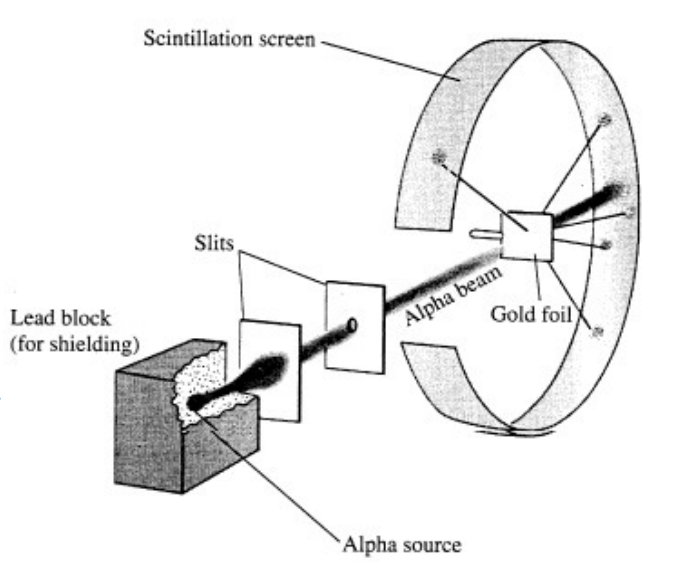
\includegraphics[scale=0.5]{Lezione1/Rutherford.png} 
\end{figure}
L'esperimento consiste nella misura del numero di particelle $\alpha$ deviate in funzione dell'angolo di deflessione:
%IMMAGINE Esp
\begin{figure}[htp!]
  \centering
  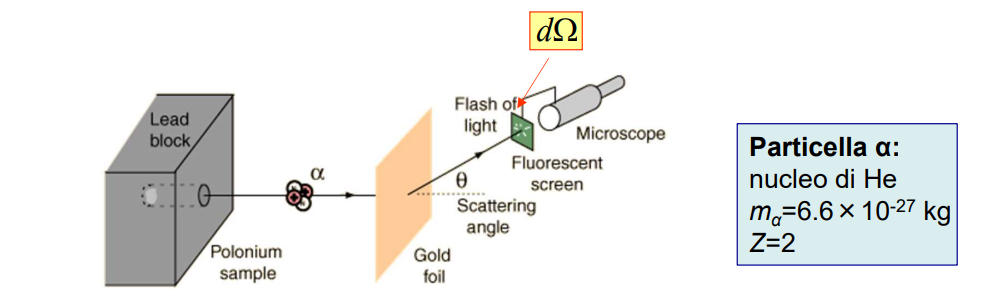
\includegraphics[scale=0.5]{Lezione1/Esp.png} 
\end{figure}
In questo esperimento è necessario determinare quantitativamente: la probabilità che una particella $\alpha$ venga deflessa in un certo angolo solido, il tasso di eventi effettivamente atteso e il concetto di \textbf{sezione d'urto}.

Si ricorda che l'angolo solido si misura in steradianti ($sr$) è l'area sottesa sulla superficie sferica di raggio unitario in analogia all'angolo in radianti ($rad$) che è l'arco sotteso sulla circonferenza di raggio unitario. Il differenziale $d\Omega$ è dato da:
\begin{equation*}
    d\Omega=\sin{\theta}d\phi d\theta\,=\, d\phi d\cos{\theta} \,=\, 2\sin{(\theta/2)}\cos{(\theta/2)}d\phi d\theta
\end{equation*}
A volte in casi di simmetria azimutale si sottointende l'integrazione su $\phi$: $d\Omega=2\pi\sin{\theta}d\theta$ e come ci si aspetta:
\begin{equation*}
    \int d\Omega=\int_0^{2\pi}d\phi\int_0^{\pi}d\theta\sin{\theta}=4\pi
\end{equation*}
Un rivelatore di area \textbf{A}, ad una distanza \textbf{r} sottende un angolo solido $\Delta\Omega=\textbf{A}/\mathbf{r^2}$
\subsection{Sezione d'urto}
In fisica nucleare e subnucleare siamo interessati a interazioni che avvengono in regioni di dimensioni inferiori a quelle di un atomo: dimensioni minori del più piccolo strumento che possiamo costruire; la stessa preparazione dello stato iniziale ha incertezze maggiori della regione in cui avvengono i fenomeni. In esperimenti di \textbf{scattering} studiamo gli \textbf{stati asintotici}: parametri \textbf{iniziali} (intensità, quantità di moto...) del fascio incidente e parametri \textbf{finali} (angolo di deflessione, quantità di moto...) del fascio delle particelle diffuse. Infatti studio il mio sistema lontano dall'interazione (molto prima e molto dopo) in quanto non posso studiare il sistema durante l'interazione. Si può misurare il tasso con cui si ottiene un certo risultato finale a partire dal sistema inizialmente preparato. Quindi, la \textbf{sezione d'urto} è una quantità collegata alla \textbf{probabilità che si verifichi un certo evento}, quindi è una quantità osservabile e interpretabile sia in meccanica classica che in meccanica quantistica.

Svolgiamo un primo esperimento ideale: prendiamo un fascio di particelle proiettile che incide su una lamina di un certo materiale. Andiamo a misurare quante particelle vengono deflesse verso un rivelatore.
%IMMAGINE ideale
\begin{figure}[htp!]
  \centering
  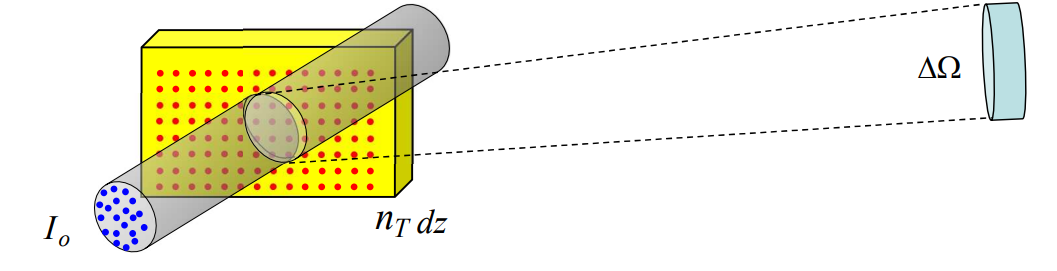
\includegraphics[scale=0.5]{Lezione1/ideale.png} 
\end{figure}
Il numero di interazioni al secondo $dn/dt$ è proporzionale a:
\begin{itemize}
    \item l'intensità del fascio (numero di particelle incidenti al secondo) $\mathbf{I_0}$;
    \item la densità di bersagli (numero di bersagi per unità di volume) $\mathbf{n_T}$;
    \item lo spessore del bersaglio $\mathbf{dz}$;
    \item l'angolo solido sotteso dal rivelatore $\mathbf{\Delta\Omega}$
\end{itemize}
\begin{equation*}
    \frac{dn(\theta)}{dt}\propto I_0\, n_T\, dz\, \Delta\Omega
\end{equation*}
La costante di proporzionalità ha le dimensioni di una superficie ed è detta \textbf{sezione d'urto differenziale} $d\sigma/d\Omega$.
\begin{equation*}
    \frac{dn(\theta)}{dt}= I_0\, n_T\, dz\, \frac{d\sigma}{d\Omega}\,\Delta\Omega
\end{equation*}

In un secondo esperimento ideale si prende un flusso di particelle proiettile che incide su dei bersagli e andiamo a misurare quante vengono deflesse verso un rivelatore (per fare un esempio concreto sulla situazione è come immaginare la terra che viene inondate da particelle provenienti dallo spazio).
%IMMAGINE ideale2
\begin{figure}[htp!]
  \centering
  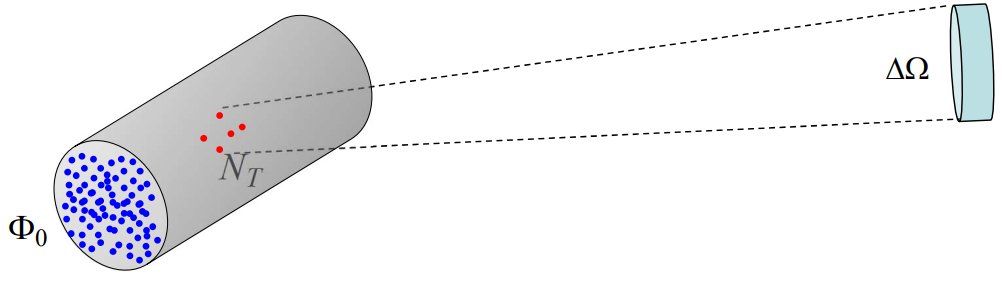
\includegraphics[scale=0.5]{Lezione1/ideale2.png} 
\end{figure}
Anche in questo caso il numero di interazioni al secondo $dn/dt$ è proporzionale a:
\begin{itemize}
    \item il flusso incidente (numero di particelle incidenti per area al secondo) $\bm{\phi_0}$;
    \item il numero di bersagli $\mathbf{N_T}$;
    \item l'angolo solido sotteso dal rivelatore $\mathbf{\Delta\Omega}$.
\end{itemize}
\begin{equation*}
    \frac{dn(\theta)}{dt}\propto \Phi_0\, N_T\, dz\, \Delta\Omega
\end{equation*}
Anche in questo caso la costante di proporzionalità ha le dimensioni di una superficie ed è detta sezione d'urto differenziale $d\sigma/d\Omega$.
\begin{equation*}
    \frac{dn(\theta)}{dt}= \Phi_0\, N_T\, \frac{d\sigma}{d\Omega}\,\Delta\Omega
\end{equation*}
Quale definizione di sezione d'urto è corretta? Le due definizioni sono \textbf{equivalenti}. Infatti se consideriamo un fascio di $\mathbf{I_0}$ particelle/s di sezione $\mathbf{S}$, che incide su un bersaglio di spessore $\mathbf{dz}$ con $\mathbf{n_T}$ atomi per unità di volume: il flusso non è altro che $\mathbf{\Phi_0=I_0}/\mathbf{S}$  e il numero di bersagli incontrati è $\mathbf{N_T=n_TdzS}$. Il numero totale di particelle deflesse nell'angolo solido $d\Omega$ sarà:
\begin{equation*}
    \frac{dn(\theta)}{dt}=\Phi_0\, N_T\, \frac{d\sigma}{d\Omega}\,d\Omega=\frac{I_0}{S}n_TdzS\frac{d\sigma}{d\Omega}d\Omega=I_0\, n_T\, dz\, \frac{d\sigma}{d\Omega}\,d\Omega
\end{equation*}
La sezione d'urto totale è: $\sigma=\int\frac{d\sigma}{d\Omega}d\Omega$
\subsubsection{Misura della sezione d'urto}
Supponiamo di poter considerare il bersaglio sottile (condizioni che si verifica molto frequentemente), ciò è equivalente alla condizione $n_Tdz\sigma<<1$. In queste condizioni per una ben definita condizione sperimentale, quindi con una fissata energia del fascio, una fissata accettanza angolare $\Delta\Omega$. Il numero $N_0$ di particele del fascio è misurata con un rivelatore \textbf{monitor}. Il numero di interazioni $n$ è misurato con il \textbf{rivelatore}.
%IMMAGINE misura
\begin{figure}[htp!]
  \centering
  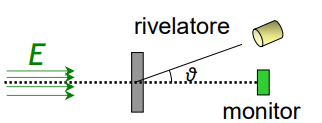
\includegraphics[scale=1]{Lezione1/misura.png} 
\end{figure}
Per fare questo devono essere conosciuti: lo spessore del bersaglio $dz$ e la densità $n_T$ di atomi/nuclei bersaglio (target)
\begin{equation*}
    n_T=\frac{\rho}{A}N_A
\end{equation*}
Dove $\rho$ è la densità, $A$ è il peso atomico e $N_A$ è il numero di Avogadro (infatti vedo che $A/N_A$ è la massa di un singolo atomo visto che il peso atomico per definizione è la massa di $N_A$ atomi). 
Piccolo inciso: ad esempio, la massa atomica del ferro è 55,847, quindi un numero di atomi di ferro pari a una costante di Avogadro (ovvero, una mole di atomi di ferro) ha una massa di 55,847 g. Viceversa, 55,847 g di ferro, contengono un numero di atomi di ferro pari a una costante di Avogadro. Quindi la costante di Avogadro corrisponde anche al fattore di conversione tra grammi (g) e unità di massa atomica (u)
La sezione d'urto allora è
\begin{equation*}
    \frac{d\sigma}{d\Omega}=\frac{1}{\Delta\Omega}\frac{1}{n_Tdz}\frac{n}{N_0}
\end{equation*}
Se gli errori su tutte le grandezze sono trascurabili escluso l'errore statistico su n, l'errore statistico sulla sezione d'urto segue la statistica di Poisson:
\begin{equation*}
    \frac{\Delta\sigma}{\sigma}=\frac{\Delta n}{n}=\frac{\sqrt{n}}{n}=\frac{1}{\sqrt{n}}
\end{equation*}
Numero di prove che hanno avuto successo su un campione molto grande di tentativi. Per cui più a lungo prendo dati migliore è la mia precisione visto che l'incertezza statistica va come $1/\sqrt{n}$.
\subsection{L'esperimento di Rutherford II}
Alla luce di quanto detto possiamo analizzare meglio l'esperimento di Rutherford. Nel modello di \textbf{Thomson} dell'atomo:
%IMMAGINE Th
\begin{figure}[htp!]
  \centering
  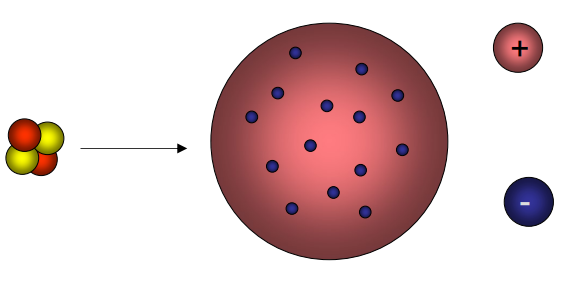
\includegraphics[scale=0.5]{Lezione1/Th.png} 
\end{figure}
sappiamo che l'elettrone è molto leggero (dall'esperimento della misura di $e/m$). Se l'urto fosse con l'elettrone $\frac{m_e}{m_\alpha}\sim10^{-4}$. Questo perchè quando un corpo molto pesante colpisce un oggetto molto leggero, il trasferimento di energia che avviene è molto piccola. L'oggetto pesante sposta via gli elettroni. Si dimostra che la massima variazione di velocità nell'urto: $|\Delta\mathbf{v}|=\frac{m_e}{2m_\alpha}\mathbf{v}$. La particella $\alpha$ non viene apprezzabilmente deviata dall'elettrone. Possiamo trascurare gli urti con gli elettroni. Ora che abbiamo escluso l'elettrone tra i ruoli importanti della deviazione della particella $\alpha$ si possono fare due ipotesi:
\begin{itemize}
    \item carica positiva uniformemente distribuita sulle dimensioni dell'atomo;
    \item carica positiva concentrata in un nucleo all'interno dell'atomo.
\end{itemize}
Dobbiamo confrontare queste due ipotesi.
\subsection{Sezione d'urto di Rutherford}
%IMMAGINE sc
\begin{figure}[htp!]
  \centering
  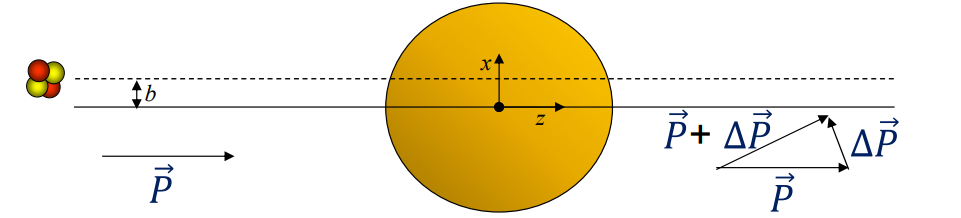
\includegraphics[scale=0.5]{Lezione1/sc.png} 
\end{figure}
Calcoliamo la sezione d'urto nel caso del processo di scattering di particella $\alpha$ con un atomo di oro. Facciamo prima delle approssimazioni (Calcolo esatto visibile in appendice (o sul Das-Ferbel)):
\begin{itemize}
    \item La particella $\alpha$ è molto veloce e l'interazione dura un tempo limitato. Questo perchè mi serve per poter assumero che il tempo di interazione sia molto piccolo e ragionare attraverso forze impulsive (quindi mi concentro solo sull'impulso totale);
    \item prima e dopo l'interazione l'energia della particella $\alpha$ è la stessa (energia potenziale nulla negli stati asintotici). Questo significa che l'interazione va a modificare solo la direzione della particella;
    \item durante l'interazione, la traiettoria devia di poco dall'andamento rettilineo dovuto al poco tempo di interazione.
\end{itemize}
Durante l'interazione la particella $\alpha$ riceve un impulso: $\Delta\mathbf{P}=\int \mathbf{F}dt$. Al termine dell'interazione essa viene deviata di un angolo: $\tan{\theta}\approx\frac{\Delta\mathbf{P}}{\mathbf{P}}$.

\subsection{Sezione d'urto elettrostatica}
Supposiamo una distribuzione di carica a simmetria sferica. L'impulso è:
\begin{equation*}
    \Delta\mathbf{P}=\int\mathbf{F}dt=\int Q_\alpha\mathbf{E}dt
\end{equation*}
Dove $Q_\alpha$ è la carica della particella $\alpha$. Nell'approssimazione in cui trascuriamo la deflessione durante l'interazione possiamo definire il \textbf{parametro di impatto} $b$, che rappresenta la distanza della traiettoria iniziale dal punto di simmetria. Invece, $v$ e $m$ sono rispettivamente la velocità (approssimazione che ci porta a dire che rimane costante) e la massa della particella $\alpha$. Quindi:
\begin{equation*}
    \Delta\mathbf{P}(b)=\int Q_\alpha\mathbf{E}(b,z)\frac{dz}{v}=\frac{Q_\alpha}{v}\int_{-\infty}^{+\infty}\mathbf{E}(b,z)dz
\end{equation*}
Dalle condizioni di simmetria ho:
\begin{itemize}
    \item $E_y(b,z)=0 \,\Rightarrow \, \Delta P_y=0$;
    \item $E_z(b,z)=-E_z(b,-z) \, \Rightarrow \,$ l'integrale su $z$ è globalmente nullo: $\Delta P_z=0$;
    \item $E_x(b,z)=E_x(b,-z)$: l'unico termine a priori non nullo è: $\Delta P_x=\frac{Q_\alpha}{v}\int_{-\infty}^{+\infty}\mathbf{E}(b,z)dz$.
\end{itemize}
Per calcolare questo integrale possiamo usare il teorema di Guass: dalle condizioni di simmetria $E_x$ non dipende dall'angolo azimutale $\phi$. Possiamo aggiungere l'integrazione su $\phi$ e dividere per $2\pi$ e quindi l'integrale diventa:
\begin{equation*}
    \Delta P_x=\frac{Q_\alpha}{v} \frac{1}{2\pi b}\int_{-\infty}^{+\infty}\int_{0}^{2\pi}E_x(b,z)dzbd\phi
\end{equation*}
L'integrale doppio non è altro che il flusso del campo elettrico attraverso il cilindro $\mathbf{C}$ di raggio $b$:
\begin{equation*}
    \int_{-\infty}^{+\infty}\int_{0}^{2\pi}E_x(b,z)dzbd\phi=\oint_C\mathbf{E}\cdot d\mathbf{S}=\frac{Q(b)}{\varepsilon_0}
\end{equation*}
Dove $Q(b)$ è la carica contenuta nel cilindro di raggio $b$. L'angolo di deflessione è quindi:
\begin{equation*}
    \tan{\theta}=\frac{\Delta P_x}{P}=\frac{Q_\alpha Q(b)}{2\pi\varepsilon_0 bv}\frac{1}{mv}=\frac{Q_\alpha Q(b)}{4\pi\varepsilon_0 bE}
\end{equation*}
Dove $E=\frac{1}{2}mv^2$ è l'energia cinetica della particella $\alpha$.

\subsubsection{Carica puntiforme}
Possiamo calcolare ora le deflessioni nei due modelli: \textbf{carica puntiforme} $Q(b)=Q_{Au}$ e quindi:
\begin{equation*}
    \tan{\theta}=\frac{Q_\alpha Q_{Au}}{4\pi\varepsilon_0 bE}
\end{equation*}
Abbiamo ricavato una relazione tra \textbf{deflessione} e \textbf{parametro di impatto}. Non c'è limite alla deflessione: tanto minore e $\mathbf{b}$, tanto maggiore è la deflessione. Infatti \textbf{sono possibili deflessioni a grandi angoli}. Si noti anche un altro aspetto generale: la deflessione diminuisce all'aumentare dell'energia infatti intuitivamente è più difficile deflettere un oggetto con una quantità di moto grande. Più un oggetto è energetico più sforzo devo fare per deviarlo.
\subsubsection{Carica distribuita uniformemente}
Ora possiamo calcolare le deflessioni nel secondo modello messo a confronto: \textbf{carica distribuita uniformemente} su un atomo sferico di raggio $\mathbf{R}$: in questo caso avrò il volume dell'intersezione con il cilindro di raggio $b<R$:
%IMMAGINE ds
\begin{figure}[htp!]
  \centering
  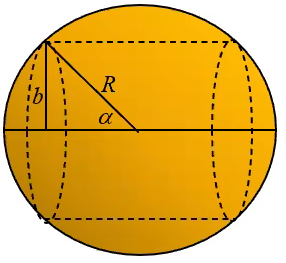
\includegraphics[scale=0.5]{Lezione1/ds.png} 
\end{figure}
\begin{equation*}
    V=\frac{4\pi}{3}(R-\sqrt{R^2-b^2})\frac{R^2+b^2-R\sqrt{R^2-b^2}}{2}+2\pi b^2\sqrt{R^2-b^2}
\end{equation*}
Il secondo termine non è altro che il volume del cilindro mentre il primo termine sono il volume delle due calotte sferiche. Viene più comodo utilizzare $\cos{\alpha}=\frac{\sqrt{R^2-b^2}}{R}$ e $\sin{\alpha}=\frac{b}{R}$:
\begin{equation*}
    V=\frac{4\pi}{3}(1-\cos{\alpha})\frac{2-\cos{\alpha}-\cos^2{\alpha}}{2}+\frac{3}{2}\sin^2{\alpha\cos{\alpha}}
\end{equation*}
Infatti è consistente con la relazione $Q(R=Q_{Au}$, $Q(0)=0$.
\begin{equation*}
    Q(b)=Q_{Au}\frac{V}{\frac{4\pi}{3}R^3}=Q_{Au}\left[ (1-\cos{\alpha})\frac{2-\cos{\alpha}-\cos^2{\alpha}}{2}+\frac{3}{2}\sin^2{\alpha\cos{\alpha}}\right]
\end{equation*}
\begin{equation*}
    \tan{\theta}=\frac{Q_\alpha Q_{Au}}{4\pi\varepsilon_0 bE}\frac{1}{\sin{\alpha}}\left[ (1-\cos{\alpha})\frac{2-\cos{\alpha}-\cos^2{\alpha}}{2}+\frac{3}{2}\sin^2{\alpha\cos{\alpha}}\right]
\end{equation*}
Si può notare che \textbf{la deflessione è massima per} $\mathbf{b=R}$, $\alpha=\pi/2$ \textbf{al diminuire di b,} $\alpha\to 0$.
Se vedo diffusione a grandi angoli significa che la prima ipotesi è quella corretta mentre la seconda ipotesi non lo è. Questa è un'osservazione qualitativa per dimostrare come l'esperimento di Ruthrford diede prova a questo.
\subsection{Sezione d'urto classica}
Usando la meccanica classica, abbiamo trovato una relazione tra il parametro di impatto $b$ e la deflessione $\theta$. Uno dei problemi è però che $b$ non è direttamente osservabile: dobbiamo trovare la sezione d'urto equivalente.

Supponiamo di avere un flusso di particelle incidente su di un atomo e deviate verso un rivelatore che copre l'angolo solido $d\Omega=\sin{\theta d\theta d\phi}$
\begin{equation*}
    \frac{dn}{dt}=\Phi\frac{d\sigma}{d\Omega}d\Omega
\end{equation*}
Da un punto di vista microscopico, le particelle deviate nell'angolo solido sono quelle che passano nell'area con i corrispondenti valori di b e $\phi$, $d\sigma=bd\phi db$.
\begin{equation*}
    \frac{dn}{dt}=\Phi bd\phi db
\end{equation*}
%IMMAGINE ss
\begin{figure}[htp!]
  \centering
  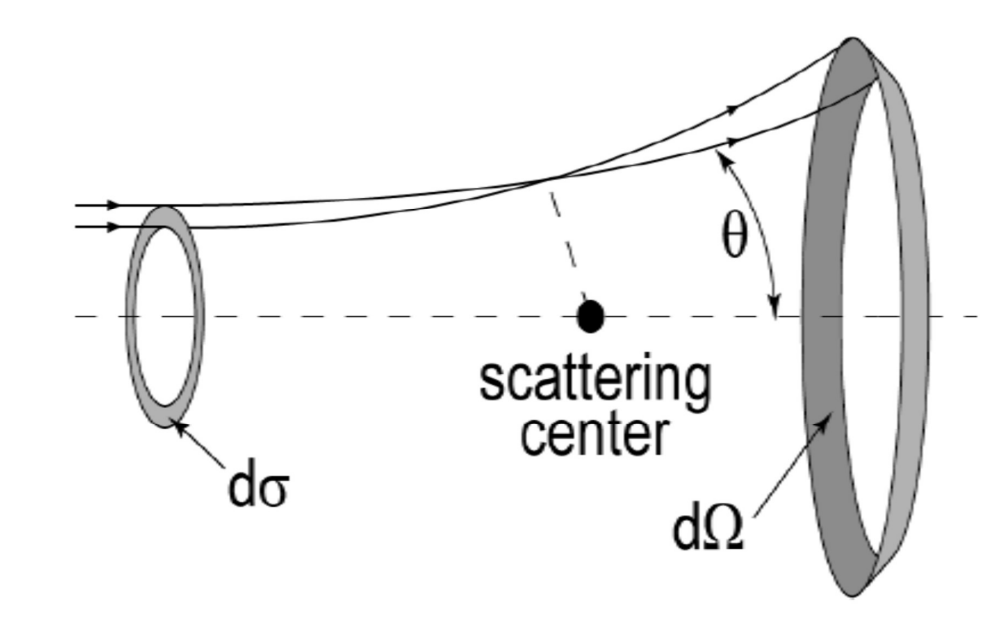
\includegraphics[scale=0.4]{Lezione1/ss.png} 
\end{figure}
Dal confronto delle due equazioni troviamo l'espressione per la sezione d'urto differenziale:
\begin{equation*}
    \frac{d\sigma}{d\Omega}=\frac{b(\theta)d\phi db}{\sin{\theta}d\theta d\phi}=\frac{b(\theta)|db/d\theta|}{\sin{\theta}}
\end{equation*}
Questa è la relazione classica per dare la definizione della sezione d'urto. Definizione che verrà utilizzata in questa lezione e basta visto che quello che tratteremo sarà tutto in ambito quantistico.
\subsection{Confronto con il modello di Thomson}
Le misure effettuate dai collaboratori di Rutherford erano in accordo con l'ipotesi di carica puntiforme. Ma potevano escludere il modello di Thomson? Sì, per effettuare il calcolo della sezione d'urto in un potenziale generico: bisogna determinare la relazione tra $b$ e $\theta$, determinare il differenziale
\begin{equation*}
    \frac{d\sigma}{d\Omega}=\frac{d\phi bdb}{d\phi \sin{\theta d\theta}}=\frac{b(\theta)}{\sin{\theta}}\frac{db}{d\theta}
\end{equation*}
%IMMAGINE grf
\begin{figure}[htp!]
  \centering
  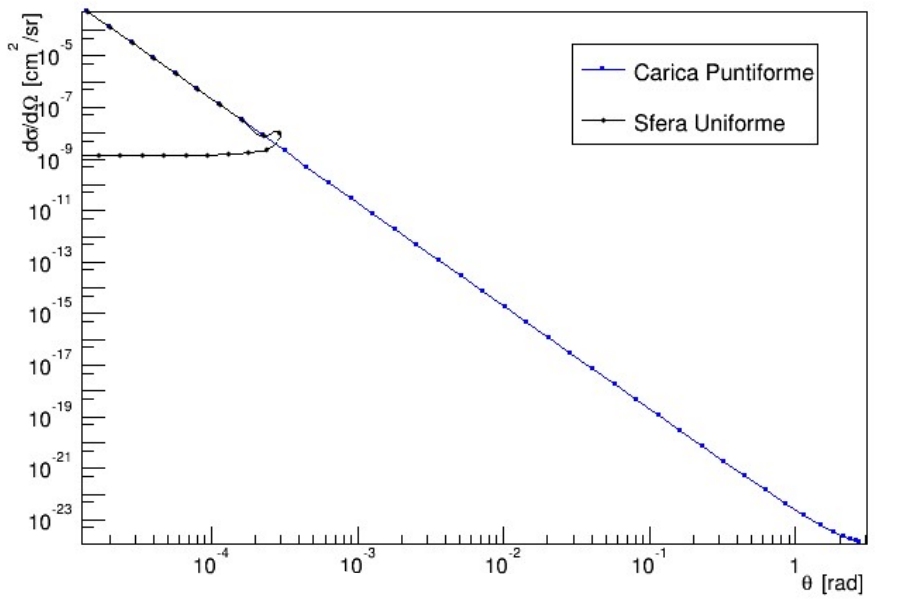
\includegraphics[scale=0.4]{Lezione1/grf.png} 
\end{figure}
Come si può osservare dal grafico si vede in funzione di $\theta$ la sezione d'urto che ci si aspetta. Nel caso di carica puntiforme c'è questa relazione in cui la sezione d'urto diminuisce molto velocemente all'aumentare di $\theta$ ma rimane comunque diversa da zero a grandi angoli (calcolo esatto non appprossimato). Per la distribuzione uniforme fino a quando siamo fuori dalla sfera l'andamento è uguale a quella puntiforme ma quando iniziamo ad entrare nella sfera la deflessione diminuisce. La sezione d'urto non continua ad estendersi ma c'è un contributo costante.
\subsection{Assorbimento e lunghezza di interazione}
La \textbf{sezione d'urto totale $\sigma$} di ottiene integrando la \textbf{sezione d'urto differenziale} su tutto l'angolo solido:
\begin{equation*}
    \sigma=\int_{0}^{2\pi}d\phi \int_0^{\pi}\sin{\theta}d\theta\frac{d\sigma}{d\Omega}
\end{equation*}
Nell'esperimento abbiamo sentito e visto una quantità che è $\frac{d\sigma}{d\Omega}$ che nel gergo viene chiamata sezione d'urto (sbagliato) questa è la sezione d'urto differenziale perchè come unità di misura è una superficie diviso l'angolo solido. Quando integro su tutto l'angolo solido passo dalla sezione d'urto differenziale ad una sezione d'urto totale diventando effettivamente un'area. 

Se io ho un fascio totale di particelle che colpisce un bersagio ho un certo numero di particelle che interagiscono. Un certo numero rispetto al numero totale del fascio di particelle. Se un fascio di particelle attraversa uno spessore $dz$: il \textbf{tasso totale} di particelle diffuse si traduce in una diminuizione dell'intensità del fascio $\mathbf{I}$:
\begin{equation*}
    \frac{dn}{dt}=-dI\,=In_Tdz\sigma \,\Rightarrow\, \frac{dI}{I(z)}=-n_T\sigma dz
\end{equation*}
Infatti il numero di particelle che interagiscono è legata ad una diminuizione del fascio. Se la diminuizione del numero di particelle nel fascio non è trascurabile, l'intensità varia con la profondità secondo la legge:
\begin{equation*}
    I(z)=I_0e^{-n_T\sigma z}=I_0e^{-\mu z}
\end{equation*}
Dove $\mu=n_T\sigma$ prende il nome di \textbf{coefficiente di assorbimento} (come unità di misura è l'inverso di una lunghezza). Analogamente si può introdurre la \textbf{lunghezza d'interazione }$\lambda$ (detta anche \textbf{libero cammino medio})
\begin{equation*}
    \lambda=\frac{1}{\mu}=\frac{1}{n_T\sigma} \qquad I(z)=I_0e^{-\frac{z}{\lambda}}
\end{equation*}
Ora posso anche capire perchè quando si parlava dell'esperimento si assumeva un bersaglio sottile, che significa $n_T\sigma dz<<1$ quindi posso trascurare la perdita, e quindi l'assorbimento del fascio.

Quindi se lo spessore $z$ è piccolo $(z<<\lambda)$ il fascio uscente è ridotto in intensità di un fattore $1-z/\lambda$ e la probabilità di scattering di una particella del fascio è $z/\lambda=n_Tz\sigma$. prodotto della desnità superficiale $n_Tz$ per la sezione d'urto $\sigma$. La sezione d'urto è legata dalla probabilità attraverso la densità superficiale dei bersagli. La densità di centri di scatterng dipende dalla densità del materiale: $n_T=\frac{\rho}{A}N_A$, spesso si esprime $\lambda$ normalizzata per la densità:
\begin{equation*}
    \lambda=\frac{1}{n_T\sigma}=\frac{A}{\rho N_A\sigma} \quad (\lambda\rho)=\frac{A}{N_A\sigma}
\end{equation*}
Questa quantità dipende dal materiale ma non dallo stato dello stesso, ha le dimensioni di una densità superficiale. Spesso viene preferita questa rispetto al libero cammino medio proprio per la comodità della non dipendenza dello stato del materiale in esame.
\subsection{Cinematica dell'urto (caso non relativistico)}
%IMMAGINE gg
\begin{figure}[htp!]
  \centering
  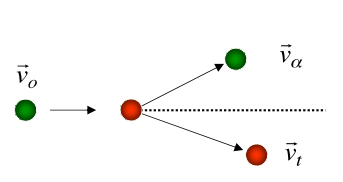
\includegraphics[scale=0.6]{Lezione1/gg.png} 
\end{figure}
Partiamo da un esperimento a bersaglio fisso in cui il bersaglio è fermo e la particella proiettile ha una certa velocità $\mathbf{v}_0$. La quantità di moto (momento) si conserva:
\begin{equation*}
    m_\alpha\mathbf{v}_0=m_\alpha\mathbf{v}_\alpha+m_t\mathbf{v}_t
\end{equation*}
\begin{equation*}
    \mathbf{v}_0=\mathbf{v}_\alpha+\frac{m_t}{m_\alpha}\mathbf{v}_t \qquad v_0^2=v_\alpha^2+\frac{m_t^2}{m_\alpha^2}v_t^2+2\frac{m_t}{m_\alpha}\mathbf{v}_t\cdot \mathbf{v}_\alpha
\end{equation*}
Si conserva anche l'energia cinetica:
\begin{equation*}
    \frac{1}{2}m_\alpha v_0^2=\frac{1}{2}m_\alpha v_\alpha^2+\frac{1}{2}m_t v_t^2
\end{equation*}
Svolgendo i conti si ottiene:
\begin{equation*}
    v_t^2\left(1-\frac{m_t}{m_\alpha}\right)=2\mathbf{v}_t\cdot\mathbf{v}_\alpha
\end{equation*}
In base a questa relazione possiamo distinguere i seguenti casi:
\begin{itemize}
    \item Se $m_t<m_\alpha$ abbiamo
\end{itemize}
%IMMAGINE ff
\begin{figure}[htp!]
  \centering
  
\includegraphics[scale=0.6]{Lezione1/ff.png} 
\end{figure}
le due particelle escono nella \textbf{stessa direzione}.
\begin{itemize}
    \item Se $m_t>m_\alpha$:
\end{itemize}
%IMMAGINE jj
\begin{figure}[htp!]
  \centering
  
\includegraphics[scale=0.6]{Lezione1/jj.png} 
\end{figure}
Le due particelle tendono ad uscire in \textbf{direzioni opposte}.
\subsection{L'esperimento di Rutherford}
Supponiamo che l'atomo abbia un nucleo molto piccolo ma molto pesante, ad esempio se consideriamo l'oro ($A=197$, $m_t\sim3.3\times10^{-25}\,kg$). Di conseguenza abbiamo $\frac{m_t}{m_\alpha}\approx50$ e quindi:
\begin{equation*}
    v_t^2\left(1-\frac{m_t}{m_\alpha}\right)=2\mathbf{v}_t\cdot\mathbf{v}_\alpha \qquad \left|v_t^2\left(1-\frac{m_t}{m_\alpha}\right)\right|=|2v_tv_\alpha\cos{\theta}|\le 2v_tv_\alpha
\end{equation*}
inoltre visto che $1-\frac{m_t}{m_\alpha}\approx-\frac{m_t}{m_\alpha}$ allora
\begin{equation*}
    v_t^2=v_\alpha^2+\frac{m_t}{m_\alpha}v_t^2 \qquad v_t\le2\frac{m_t}{m\alpha}v_\alpha
\end{equation*}
Inoltre andando a fare la parte sull'energia:
\begin{equation*}
    v_0^2=v_\alpha^2+\frac{m_t}{m_\alpha}v_t^2 \le v_\alpha^2+\frac{m_t}{m_\alpha}\left(2\frac{m_\alpha}{m_t}\right)^2v_\alpha^2=v_\alpha^2+4\frac{m_\alpha}{m_t}v_\alpha^2 \approx v_\alpha^2
\end{equation*}
Pertanto il momento del nucleo \textbf{dopo} l'urto è:
\begin{equation*}
    v_t\le2\frac{m_\alpha}{m_t} \quad m_tv_t\le 2m_\alpha v_\alpha \quad m_tv_t\le2m_\alpha v_0
\end{equation*}
dato che prima abbiamo visto che $v_\alpha\approx v_0$. Significa che la particella $\alpha$ può addirittura rinculare indietro.
\subsection{Il sistema del centro di massa}
Il centro di massa si muove con velocità $\mathbf{v}_{cm}=\frac{\mathbf{p}_{tot}}{m_{tot}}=\frac{m_\alpha\mathbf{v}_0+m_t 0}{m_t+m_\alpha}$. Il sistema del centro di massa è quello in cui il centro di massa è in quiete. In questo sistema, prima dell'urto, proiettile e bersaglio hanno velocità:
\begin{equation*}
    \mathbf{v}_\alpha^{*}=\mathbf{v}_0-\mathbf{v}_{cm}=\frac{m_t}{m_t+m_\alpha}\mathbf{v_0}\qquad \mathbf{v}_t^{*}=-\mathbf{v}_{cm}=-\frac{m_\alpha}{m_t+m_\alpha}\mathbf{v}_0
\end{equation*}
e come ci aspettiamo:
\begin{equation*}
    \mathbf{p}_\alpha^{*}=m_\alpha\mathbf{v}_\alpha^{*}=-\mathbf{p}_t^{*}=-m_t\mathbf{v}_t^{*}\to\mathbf{p}_{tot}^{*}=0
\end{equation*}
Mentre le energie cinetiche sono:
\begin{equation*}
    T_\alpha^{*}=\frac{p_\alpha^{*}}{2m_\alpha} \qquad T_t^{*}=\frac{p_t^{*}}{2m_t}
\end{equation*}
ma $|p_\alpha^{*}|=|p_t^{*}|$ e quindi $T_\alpha^{*}/T_t^{*}=m_t/m_\alpha$. In questo sistema nell'urto non cambia il modulo delle velocità, il momento e l'energia. L'unico grado di libertà è l'angolo di deflessione $\theta^{*}$. Dopo l'urto: $|\mathbf{v}_\alpha^{'*}|=|\mathbf{v}_\alpha^{*}|$ e $\mathbf{v}_\alpha^{'*}\cdot\mathbf{v}_\alpha^{*}=v_\alpha^{*2}\cos{\theta^{*}}$